\documentclass[a4paper,12pt, twoside]{article} 
\usepackage[french]{babel}
\usepackage[utf8]{inputenc}
\usepackage{answers}

\usepackage{hyperref}

\usepackage[table,xcdraw]{xcolor}
\usepackage{listings}
\definecolor{ForestGreen}{RGB}{34,139,34}

\usepackage{multicol}

\usepackage{enumitem}

\newcommand{\py}{\lstinline{Python} }

%%%%%%%%%%%%%%%%%%%%%%%%%%%%%%%% CONSTANTES %%%%%%%%%%%%%%%%%%%%%%%%%%%%%%%%%%%
\newcommand{\numero}{4}                                    %Numéro de la série -1
\newcommand{\titreserie}{Stockage de données}  

\definecolor{backcolour}{rgb}{0.95,0.95,0.92}

\lstset{%
	language         = Python,
	backgroundcolor  = \color{backcolour},
	basicstyle       = \ttfamily, % \upshape\ttfamily,
	keywordstyle     = \bfseries\color{blue}, %\bfseries,
	stringstyle      = \color{magenta},
	commentstyle     = \color{ForestGreen},
	alsoletter = > ,
	morekeywords = {>>>,as,assert,False,None, nonlocal,True, with,yield},
	showstringspaces = false,
	numbers=left,
	stepnumber=1,
	literate={à}{{\`{a}}}1 {é}{{\'e}}1 {è}{{\`{e}}}1 {ê}{{\^{e}}}1 {ç}{{\c{c}}}1 {Ç}{{\c{C}}}1,
}

\newcommand{\itemb}[1]{\item \textbf{#1}}

\usepackage{fancyhdr}  %package pour en-tetes et pied de pages
\usepackage{sectsty} % Permet de faire des modifications de police dans diverses sections des "headings" (cf. modif presentation de la page)
\pagestyle{fancy}       %Style pour en-tetes et pieds de pages
\fancyhead[CO,CE]{\sc Série 4\hspace{0.5mm}}
\fancyhead[RO,LE]{Collège Sismondi}  % LaTeX/TEX define \strut to be an invisible box of width zero that extends just enough above and below the baseline. Cela permet d'augementer légèrement la taille en bas de la box de manière à ce qu'elle soit collée à la ligne.
\fancyhead[LO,RE]{\small\ \textsl{1\textsuperscript{er} année - Informatique}}
\fancyfoot[RO,LE]{2021 - 2022}
\fancyfoot[LO,RE]{\small M.Schiess }
\fancyfoot[CO,CE]{\thepage}

\fancyhfoffset[l]{1.2cm} % le "l" en paramètre permet d'indiquer qu'on ne veut modifier que la marge à gauche.
\renewcommand{\headrule}{{%
		\hrule \headwidth \headrulewidth \vskip-\headrulewidth}}
\renewcommand\footrulewidth{\headrulewidth}
\renewcommand{\footrule}{{%
		\vskip-\footruleskip\vskip-\footrulewidth
		\hrule \headwidth \footrulewidth\vskip\footruleskip}}

\usepackage{tikz}
%-------------------------------------------------------------------------------
%---- Eclairage : en encadré sur fond jaune avec symbôle "ampoule" à gauche ----
%-------------------------------------------------------------------------------
\definecolor{coleclairage}{RGB}{255 , 221 , 156}
\definecolor{contoureclairage}{RGB}{255 , 192 , 0}
\newenvironment{eclairage}
{
	\begin{center}%
		\begin{tikzpicture}%
			\node[rectangle, draw=contoureclairage, top color=coleclairage!50, bottom color=coleclairage!140, rounded corners=5pt, inner xsep=5pt, inner ysep=6pt, outer ysep=10pt]\bgroup                     
			\begin{minipage}{0.98\linewidth}
				\begin{minipage}{0.08\linewidth}\centerline{
\includegraphics[scale=1]{../../theorie/Images/Symbole_eclairage.png}}\end{minipage}
				\begin{minipage}{0.89\linewidth}\itshape\footnotesize
				}
				{                		
				\end{minipage}
			\end{minipage}\egroup;%
		\end{tikzpicture}%
	\end{center}%
}

%-------------------------------------------------------------------------------
%---- apprendre : en encadré sur fond jaune avec symbôle "ampoule" à gauche ----
%-------------------------------------------------------------------------------
\definecolor{colapprendre}{RGB}{50,205,50}
\definecolor{contourapprendre}{RGB}{34,139,34}
\newenvironment{apprendre}
{
	\begin{center}%
		\begin{tikzpicture}%
			\node[rectangle, draw=contourapprendre, top color=colapprendre!10, bottom color=colapprendre!50, rounded corners=5pt, inner xsep=5pt, inner ysep=6pt, outer ysep=10pt]\bgroup                     
			\begin{minipage}{0.98\linewidth}
				\begin{minipage}{0.08\linewidth}\centerline{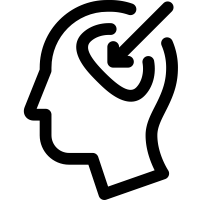
\includegraphics[width=30px]{../../theorie/Images/Symbole_learn.png}}\end{minipage}
				\begin{minipage}{0.89\linewidth}\itshape\footnotesize
				}
				{                		
				\end{minipage}
			\end{minipage}\egroup;%
		\end{tikzpicture}%
	\end{center}%
}


%-----------------------------------------------------------------
%---- Modification présentation de la page: marges de la page ----
%-----------------------------------------------------------------
%\addtolength{\hoffset}{-1in}              % 1
%\addtolength{\voffset}{-1in}              % 2
\addtolength{\oddsidemargin}{-0.1 in} % 3
\addtolength{\evensidemargin}{-1in} % 3
\addtolength{\topmargin}{-1in}       % 4
\addtolength{\headheight}{6pt}       % 5
%\addtolength{\headsep}{-0.2cm}           % 6
\setlength{\textheight}{26cm}    % 7
\setlength{\textwidth}{16.5cm}      % 8
\addtolength{\marginparsep}{0pt}      % 9
\setlength{\marginparwidth}{0pt}   % 10
\addtolength{\footskip}{-1mm}           %11

\setlength{\parindent}{0em}% pas d'indentation


% Customiser le nom des sections
\usepackage{titlesec}
\titleformat{\section}[hang]{\Large \bfseries}{Série \thesection:\ }{0pt}{}

\renewcommand{\familydefault}{\sfdefault} % pour avoir des polices san serif

\newtheorem{Exc}{Exercice}
\Newassociation{correction}{Soln}{mycor}
\renewcommand{\Solnlabel}[1]{\bfseries Ex #1 }
\def\exo#1{%
	\futurelet\testchar\MaybeOptArgmyexoo}
\def\MaybeOptArgmyexoo{
	\ifx[\testchar \let\next\OptArgmyexoo
	\else \let\next\NoOptArgmyexoo \fi \next}
\def\OptArgmyexoo[#1]{%
	\begin{Exc}[#1]\normalfont}
	\def\NoOptArgmyexoo{%
		\begin{Exc}\normalfont}
		\newcommand{\finexo}{\end{Exc} \vspace{3mm}}
	\newcommand{\flag}[1]{}
	\newcommand{\entete}[1]

\newcommand{\getexocompteur}{{\the\numexpr \arabic{Exc}  \relax}}	
	
\newcommand{\eexo}{\vspace{5mm}} % espace pour séparer les exercices

\begin{document}
%		\title{\vspace{-3cm}Série 1}
%		\date{\vspace{-2cm}}
%		\maketitle

\fancyhead[CO,CE]{\sc Série \arabic{section} \hspace{0.5mm}}

\setcounter{section}{\numero}
\section{\titreserie}				
\Opensolutionfile{mycor}[cor_01]

\exo{}[Donnée format et taille]  ~\\ 
	\begin{enumerate}
		\item Créer un document avec \textit{Libre office writer} contenant le texte : \newline


		\begin{minipage}{1\linewidth}
			\texttt{Je ne contient pas beaucoup d'informations mais en fonction de mon format, j'ai besoin de plusieurs milliers d'octets pour être stocké!\\
		}
	
		Sauvegarder le document dans le format libre office (Text ODT).
		
		\item Depuis libre office , utilisez le menu "\textit{fichier}" et "\textit{enregistrer sous}" pour sauvegarder le fichier, en 
			\begin{itemize}
				\item \textit{Rich text format}, extension rtf;
				\item en fichier texte standard, extension txt.
			\end{itemize}
		\end{minipage}
	
		\item Utiliser l'explorateur de fichier pour déterminer la taille en octet de chacun des 3 fichiers.
		
		\item Ces trois fichiers sont-ils des fichiers textes comme nous l'avons défini au chapitre précédent? Pour répondre à cette question, ouvrir chacun des fichiers avec une éditeur de texte (par exemple \textit{kate}).
		
	\end{enumerate}

	\begin{correction}
	~\\ 
	La taille des fichiers est la suivante (avec la version de Libre office que j'ai à la maison)
	\begin{itemize}
		\item \lstinline{exemple_texte.txt} : 146 octets
		\item \lstinline{exemple_texte.rtf} : 2,3 octets, c'est un fichier texte qui contient des information de mis en page.
		\item \lstinline{exemple_texte.odt} : 9,3 Ko, c'est un fichier binaire.
	\end{itemize}
\end{correction}
\finexo


\exo{}[Taille d'un fichier texte]  ~\\ 
	En vous basant sur ce que vous avez appris cette année enb informatique, essayez de calculez la taille que ferait un fichier texte \texttt{blabla.txt} contentant la chaîne de caractères \texttt{blablabla}.
	Comparer ensuite en le créant  sur votre ordinateur.
	\begin{correction}
		~\\ 
		La chaîne de caractères \texttt{blablabla} contient 9 caractères donc au minimum 9 octets.
	\end{correction}
\finexo

\exo{}[Taille d'un livre]  ~\\ 
Combien d'octets contient le livre que vous lisez en français
\begin{correction}
	~\\ 
	Regardez combien de caractères il y a environ sur une ligne et combien il y a de lignes par page. Vous multiplier ces deux nombres pas le nombre de pages et vous aurez une estimation du nombre d'octets nécessaire pour stocker le livre
\end{correction}
\finexo

\exo{}[compression sans perte de donnée]  ~\\ 
	Depuis le moodle du cours, téléchargez le livre	\lstinline{Discours_de_la_methode_Descartes.txt}. Compressez-le en zip et comparez sa taille originale avec sa taille une fois compressé.
	\begin{correction}
		~\\ 
		Non compressé le livre fait 125.3 Ko et l'archive zip fait 39.6 Ko.
	\end{correction}
\finexo

\exo{}[Image format, taille et compression]  ~\\ 
Le but de cet exercice est de comparer la taille et la qualité d'une image en fonction du format d'encodage. 

Pour convertir les images, on va utiliser le programme en ligne de commande ImageMagic:
\begin{enumerate}
	\item Depuis le moodle du cours à la section "5. Stockage de données", téléchargez l’image sous le nom \texttt{disney.bmp} dans le dossier de votre choix (par exemple "Document"). 
	\item Avec l'explorateur de fichier "Dolphin", allez dans le dossier où l'image \texttt{disneyb.bmp} a été téléchargée puis \textbf{pressez la touche "F4" pour ouvrir un terminal de commande.}
	
	Pour information la résolution de l'image est de 548 par 390 (les dimensions du tableau de pixel) et chaque couleur est codée sur 24 bits.
	
	\item On veut réduire la qualité de l'image en diminuant le nombre de couleurs nécessaire pour représenter les couleurs. Dans l'image d'origine, la couleur de chaque pixel est représenté sur 24 bits ($2^24$ possibilités), un octet pour chaque composante R (red), G (green) et B (blue).	
	
	\vspace{2mm}
	
	Pour convertir l'image téléchargée en format bmp avec les couleurs codés sur 8 bits (1 octet), on tape, dans le terminal, la commande
	\begin{lstlisting}[numbers=none]
		convert -colors 4 disney.bmp disney_4b.bmp
	\end{lstlisting}
	
	\item On veut compresser l'image (avec perte d'information). On utilise deux formats de compression le "png" et le "jpg".
	
	\vspace{2mm}
	
	Utilisez les commandes suivantes:
	\begin{lstlisting}[numbers=none]
		convert -quality 10  disney.bmp disney.jpg
		convert -quality 10  disney.bmp disney.png
	\end{lstlisting}
	Le paramètre \lstinline{-quality 10} permet d'ajuster le niveau de compression.
	
	\item On va diviser les dimensions de l'image par deux avec la commande
	\begin{lstlisting}[numbers=none]
		convert -resize 50%  disney.bmp disney_petite.bmp
	\end{lstlisting}
	\item Compléter le tableau suivant
	\begin{center}
		\begin{tabular}{| l || c | r | }
			\hline
			Format & Taille (ko) & Qualité visuelle \\ \hline
			.bmp en 24 bits &  &  \\ \hline
			.bmp en 24 bits 2 fois plus petite &  &  \\ \hline
			.bmp en 4 bits &  &  \\ \hline
			.jpg &  &  \\ \hline
			.png &  &  \\
			\hline
		\end{tabular}
	\end{center}
	\item Pourquoi l'image \texttt{disney\_petite.bmp} prend 4 fois de place que l'image d'origine.
	\vspace{2cm}
	\item Sachant que les dimensions de l'images sont 548 x 390 et que chaque pixel est codé sur 24 bits (3 octets), estimer par un calcul la taille de l'image sans aucune compression.
	\vspace{2cm}
	\item \textbf{Faire une copie de toutes les images sur votre drive dans le dossier exercice.}
\end{enumerate}


\begin{correction}
	~\\ 
	\begin{enumerate}
		\item Relire éventuellement le chapitre sur la navigation dans l'arborescence du chapitre précédent.
		\item \ 
		\item L'image originel fait 641.3 Ko ce qui est cohérent car il y a 548 x 390= 213720 pixels et 3 octets par pixels (couleurs codés sur 24 bits) ce qui fait en tout 213720 x 3 = 641160 octets = 641.16 Ko (les méta-données doivent expliquer la différence). Pour l'image avec les couleurs codés sur 8 bits=0.5 octet l'image fait 107,8 ce qui est cohérent avec le calcul 213720 x 0.5 = 106860 octets.
		\item Il y une perte de qualité.
		\item Il y a 4 fois mois de pixels donc l'image prend 4 fois moins de place.
		\item \ \newline
		\begin{center}
			\begin{tabular}{| l || c | r | }
				\hline
				Format & Taille (ko) & Qualité visuelle \\ \hline
				.bmp en 24 bits & 641.3Ko  & bonne \\ \hline
				.bmp en 24 bits 2 fois plus petite & 160.8Ko & moins bonne résolution \\ \hline
				.bmp en 4 bits & 107.8 & moins de couleurs \\ \hline
				.jpg & 8Ko & mauvaise qualité \\ \hline
				.png & 14.3Ko & qualité moyenne \\
				\hline
			\end{tabular}
		\end{center}
		\item Si on divise par deux la taille du tableau de pixels le nombre de pixels va être divisé par 4.
		\item En octets : $548 \cdot 390 \cdot 3 = 641'160\ [ 0 ] = 641\ [ko]$, si on ajoute les méta-données (dimension de l'image, code couleurs, etc... ) on est proche du nombre 641.3Ko.
	\end{enumerate}
	\newpage
\end{correction}
\finexo

\cleardoublepage

% Solution		

		\setcounter{page}{1}
		\setcounter{section}{\numero}
		\Closesolutionfile{mycor}
		\titleformat{\section}[hang]{\Large \bfseries}{Corrigé Série \thesection:\ }{0pt}{}
		

		\fancyhead[CO,CE]{\sc Corrigé Série \arabic{section} \hspace{0.5mm}}
		\section{}
		\Readsolutionfile{mycor}
	\end{document}